%!TEX root = ../terrainbook.tex
% chktex-file 46

% \setchapterpreamble[u]{\marginnote[12pt]{\faVideoCamera\ \url{https://youtu.be/_BSuNu3Ahw0}}\margintoc[18pt]}
\setchapterpreamble[u]{\margintoc}
% \setchapterpreamble[u]{\margintocvideo[0mm]{https://youtu.be/_BSuNu3Ahw0}}
\chapter{What is a terrain?}%
\label{chap:whatisterrain}
\labch{whatisterrain}

\graphicspath{{whatisterrain/}}



%%%%%%%%%%%%%%%%%%%%%%%%%%%%%%%%%%%%%%%%%%%%%%%%%%%
% DTM == representation of the Earth's surface
% Dimensionality of DTM (2D, 2.5D, 2.75D, 3D)
% DTM, DSM, DEM
% nDSM: https://www.stadtentwicklung.berlin.de/umwelt/umweltatlas/ed610_03.htm
% Representation of DTMs in computers
%   - a DTM is a 2D field (object vs field discussion from GEO1002)
%   - 6 common representations: regularly spaced sample points; irregularly spaced sample points; contour lines; rectangular cells (raster); triangulated irregular networks (TIN); planar partition with arbitrary polygons.
%   - some are incomplete
%   - discussion data model vs data structure?




% \begin{center}
%   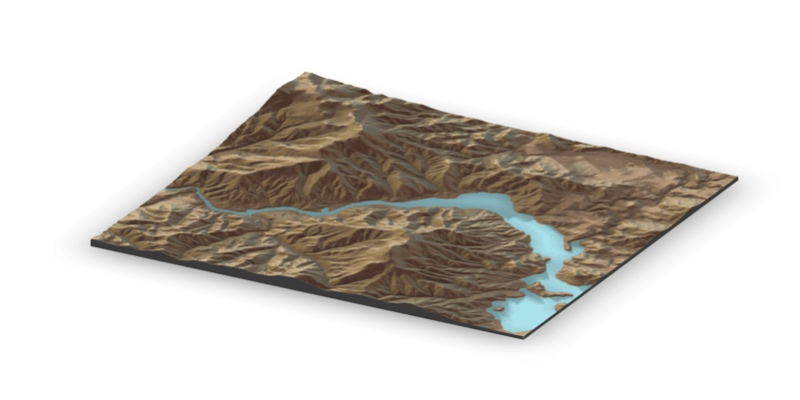
\includegraphics[width=0.95\linewidth]{figs/header.jpg}
% \end{center}

Defining what a terrain, also called a \emph{digital terrain model} (DTM), is not simple because there is no universal agreement, neither among practitioners nor in the scientific literature.
Different terms are used, often interchangeably.

In most cases, we can state that:

\begin{quote}
A terrain is a representation of the Earth's surface. 
It gives us the \emph{elevation}, which is the height above/below a certain reference point (a vertical datum)
\end{quote}

However, the ``Earth's surface'' is also not a clear concept, since several objects on it can be present, \eg\ man-made structures like buildings, roads, power lines, and bridges, and other objects like trees.

\begin{marginfigure}
  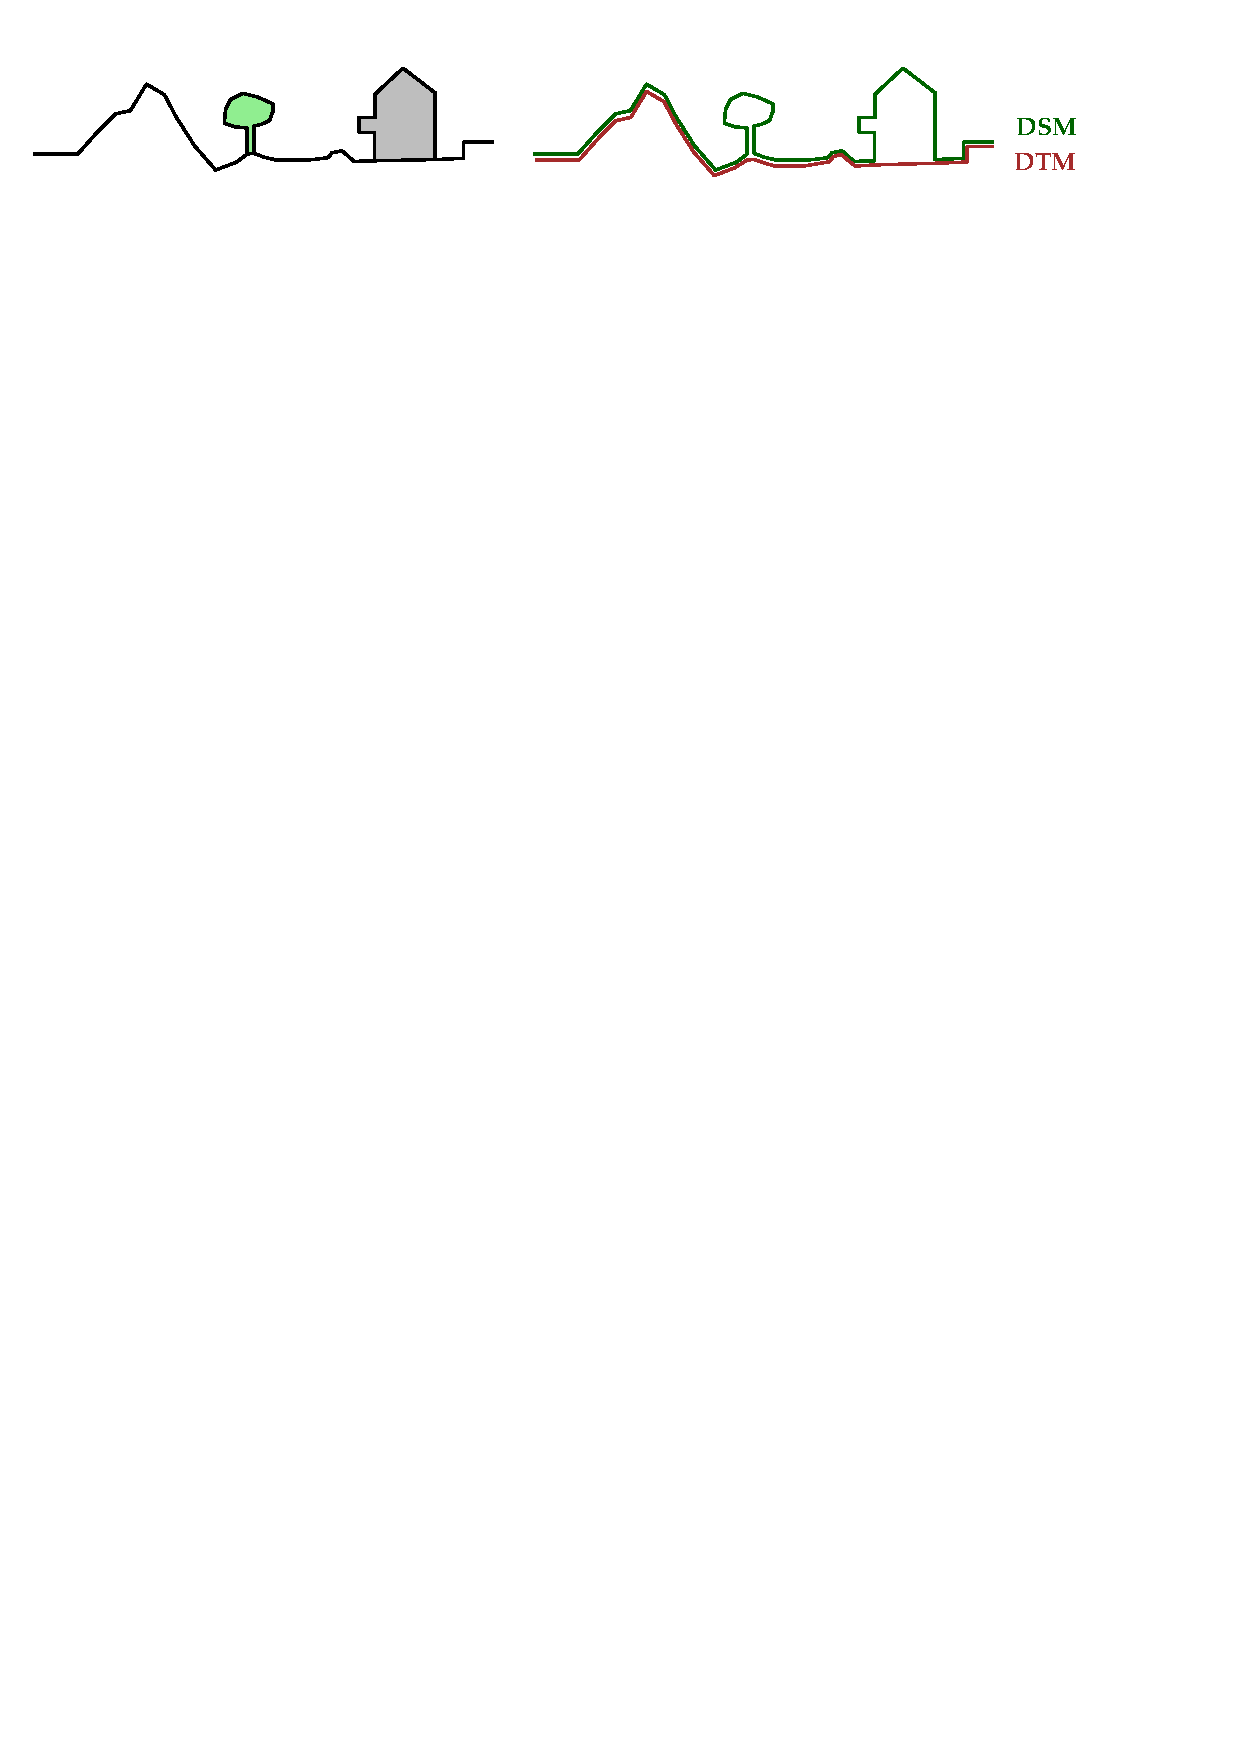
\includegraphics{figs/dtmdsm}
  \caption{\textbf{Top}: a terrain with a mountain, a tree, and a building. \textbf{Bottom}: its DSM and DTM.}%
\labfig{fig:dtmdsm}
\end{marginfigure}
We use the following definitions in this course (see \reffig{fig:dtmdsm}):
\begin{description}
  \item[DEM] (\textbf{D}igital \textbf{E}levation \textbf{M}odel). In the literal meaning of the term, it is simply a model of the elevation. A DEM is either a DSM or a DTM\@.\index{DEM} 
  \item[DTM] (\textbf{D}igital \textbf{T}errain \textbf{M}odel). The surface of the Earth is the \emph{bare-earth}, that is no man-made objects or vegetation is present. 
  \item[DSM] (\textbf{D}igital \textbf{S}urface \textbf{M}odel). The surface includes all objects and structures on the terrain.\index{DSM}
\end{description}

It should be noticed that in some countries a DEM is often synonymous with a grid of elevation (see below).


%%%
%
\section{Dimensionality of DTMs}

The term ``3D'' is misleading in a DTM context, as it is in a GIS context, because it might refer to three different concepts: 2.5D, 2.75D, and 3D (see \reffig{fig:dimgis}).
\begin{figure*}[b]
  \centering
  \begin{subfigure}[b]{0.45\linewidth}
    \centering
    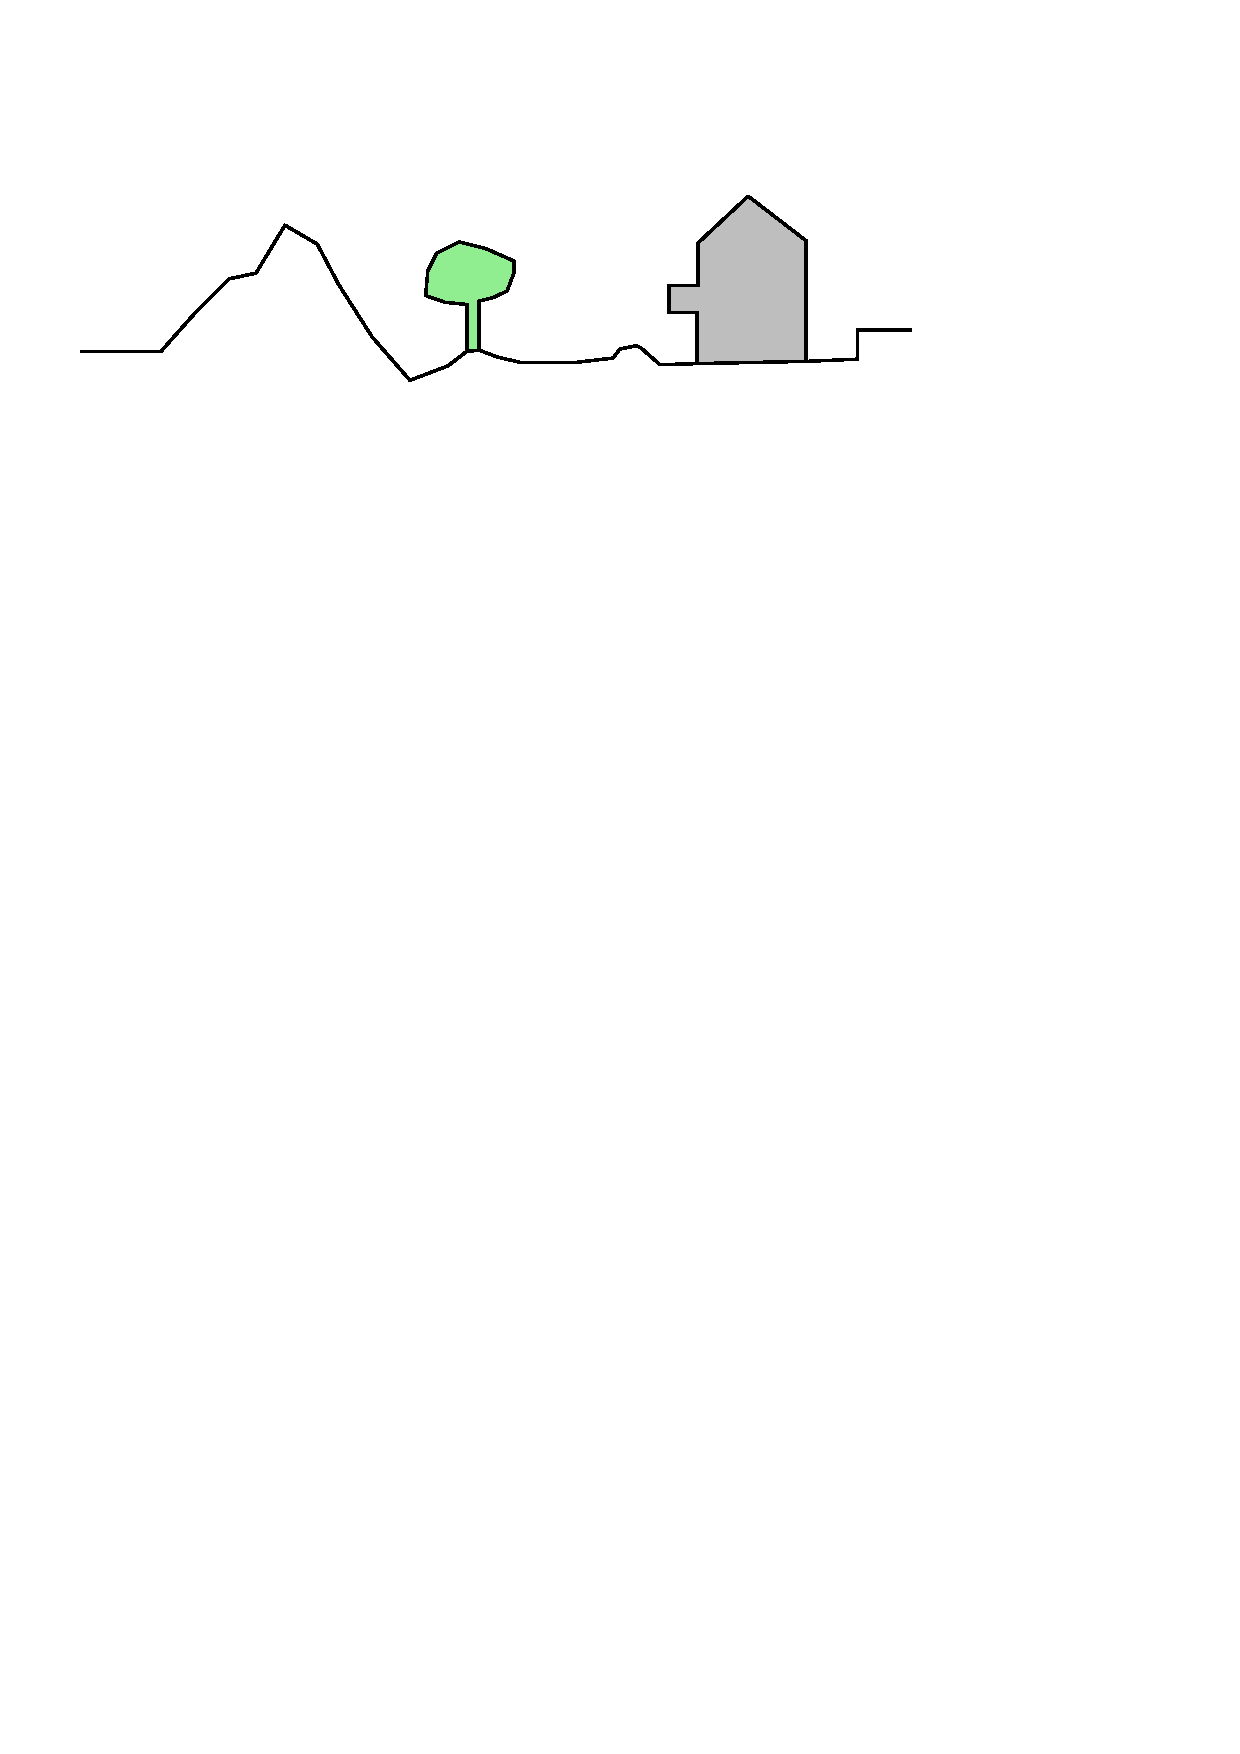
\includegraphics[page=1,width=\linewidth]{figs/dimgis}
    \caption{A terrain}\labfig{fig:dimgis:1}
  \end{subfigure}%
  \qquad %-- that adds some space between th 2 figures
  \begin{subfigure}[b]{0.45\linewidth}
    \centering
    \includegraphics[page=6,width=\linewidth]{figs/dimgis}
    \caption{2.5D modelling}\labfig{fig:dimgis:25}
  \end{subfigure}%
  \qquad %-- that adds some space between th 2 figures
  \begin{subfigure}[b]{0.45\linewidth}
    \centering
    \includegraphics[page=5,width=\linewidth]{figs/dimgis}
    \caption{2.75D modelling}\labfig{fig:dimgis:275}
  \end{subfigure}%
  \qquad %-- that adds some space between th 2 figures
  \begin{subfigure}[b]{0.45\linewidth}
    \centering
    \includegraphics[page=4,width=\linewidth]{figs/dimgis}
    \caption{Volumetric modelling, or full 3D}\labfig{fig:dimgis:3}
  \end{subfigure}%
  \caption{Different meanings for `3D GIS' in the context of terrains.}
\labfig{fig:dimgis}
\end{figure*}


\subsection{2.5D}%
\index{2.5D} 
What is usually used for modelling terrains: a surface (which is a topologically a 2D object; also called a 2-manifold) is embedded in 3D space, and each location ($x,y$) is assigned to one and only one height $z$.
% \marginnote{Text of the note}
In other words, the surface can be projected to the $xy$-plane and maintain its topology.
When we refer to terrains in this course, this is what is usually mean, unlike explicitly stated otherwise.
This is often what is used in GIS software, and both the well-known raster/grid  is such a case.
Observe that this restricts the real-world cases that can be modelled because, as shown in \reffig{fig:dimgis}b, vertical surfaces (\eg\ walls of a building if we model all man-made objects with the terrain to construct a digital surface model), overfolds (\eg\ the balcony of a house) and caves are impossible to represent.
As shown in the figure, these are modelled as nearly vertical surfaces; in practice the wall of building could deviate by for instance 1 degree from the vertical. 

\subsection{2.75D}%
\index{2.75D} 
This also refers to a surface (a 2-manifold) but unlike for the 2.5D case, the surface is not restricted to be projectable to the 2D plane (see \reffig{fig:dimgis}c).
Thus, more than one $z$ value is allowed for a given location ($x,y$).
The term '2.75D' was coined because: it is more than 2.5D, but less than 3D.
The surface represents the exterior of all objects/features together, and vertical walls are allowed.
Surface modelling is popular in CAD, but in the GIS it is rather rare.
We are not aware of any popular GIS software that allows us to model a terrain as a 2.75D and perform operations on it.

\subsection[3D]{Full 3D, or volumetric modelling} 
This refers to the modelling of not only the boundaries of objects, but also of the interior of these.
Notice for instance in \reffig{fig:dimgis}d that each building is represented with a solid.
The volume of buildings can therefore be calculated (since the ground floor of buildings would be modelled for instance), while with the other variations it is not possible. 
Such a representation is usually done with a 2.5D terrain (although a 2.75D could also be used) and a set of buildings/objects that are connected to the terrain.



%%%
%
\section{2.5D terrain == field}

In the context of this course, we assume that a terrain is a 2.5D object, and therefore a terrain can be considered as a \emph{field}.%
\index{field}\marginnote{field}
A field is a model of the spatial variation of an attribute $a$ over a spatial domain, which in our case is $\mathbb{R}^2$, the two-dimensional Euclidean space.
It is modelled by a function mapping one point $p$ in $\mathbb{R}^2$ to the value of $a$, thus 
\[
  a = f(p)
\]
The function can theoretically have any number of independent variables, but in the context of a terrain the function is usually bivariate ($x,y$).

%

The representation of a field in a computer faces many problems. 
First, fields are continuous functions, and, by contrast, computers are discrete machines. 
Fields must therefore be \emph{discretised}, \ie\ broken into finite parts.
\index{discretisation}\marginnote{discretisation}
Second, in practice it is usually impossible to measure continuous phenomena everywhere, and we have to resort to collecting samples at some finite locations and reconstructing fields from these samples.
The discretisation task therefore begins at the acquisition phase, and is affected by the acquisition tools and techniques (more about this in \refchap{chap:acquisition}).
This fact is aggravated for fields as found in GIS-related disciplines because, unlike disciplines like medicine or engineering, we seldom have direct and easy access to the whole object of interest.


%%%
\subsection{What is needed to represent a field/terrain?}

To represent a terrain in a computer, and be able to manipulate it (\ie\ edit the terrain and extract information such as slope), two things are needed:
\begin{enumerate}
  \item a set of samples that were collected to study the terrain, for instance a point cloud obtained from airbone laserscanning or photogrammetry (see \refchap{chap:acquisition} for details).
  \item a set of rules to obtain one and only one elevation value at any location ($x,y$); in other words, to reconstruct the continuity of the surface from the discrete samples.
  This operation is referred to as spatial interpolation (Chapters~\ref{chap:interpol} and~\ref{chap:kriging}). 
\end{enumerate}


%%%
\subsection{Strategy \#1: points + global interpolation function.}
This means storing the original sample points with the parameters of the \emph{global} spatial interpolation method that is best suited to the distribution of the samples and their accuracy.
Global methods are for instance inverse-distance to a power, natural neighbours, or Kriging.
This strategy is used because one can compactly represent a field (only the samples and a few parameters need to be stored).

Notice that this strategy permits us to reconstruct the continuity of a terrain from the samples by calculating the value of the elevation, but that this value is \emph{not} persistently stored in memory.
It is therefore less used in practice than the next strategy, which allows us to permanently store the terrain in a file and avoids us recomputing every time al the needed elevation values.


%%%
\subsection{Strategy \#2: piecewise spatial models}
This means that the spatial interpolation function used is \emph{piecewise} (instead of being global).
\marginnote{piecewise function}\index{piecewise function}
That is, the two-dimensional domain of the terrain (the $xy$-plane) is tessellated, or partitioned, into several pieces, and for each of these we assign an interpolation function describing the spatial variation in its interior.
This function is usually a simple mathematical function:
\begin{itemize}
  \item constant function: the value of the modelled attribute is constant within one cell;
  \item linear function;
  \item higher-order function.
\end{itemize}

%

In general, we  classify the tessellations of space into three categories (as shown in \reffig{fig:tesstypes}): \emph{regular}, \emph{irregular}, and \emph{hierarchical}.%
\index{tessellation}
\begin{marginfigure}
  \centering
  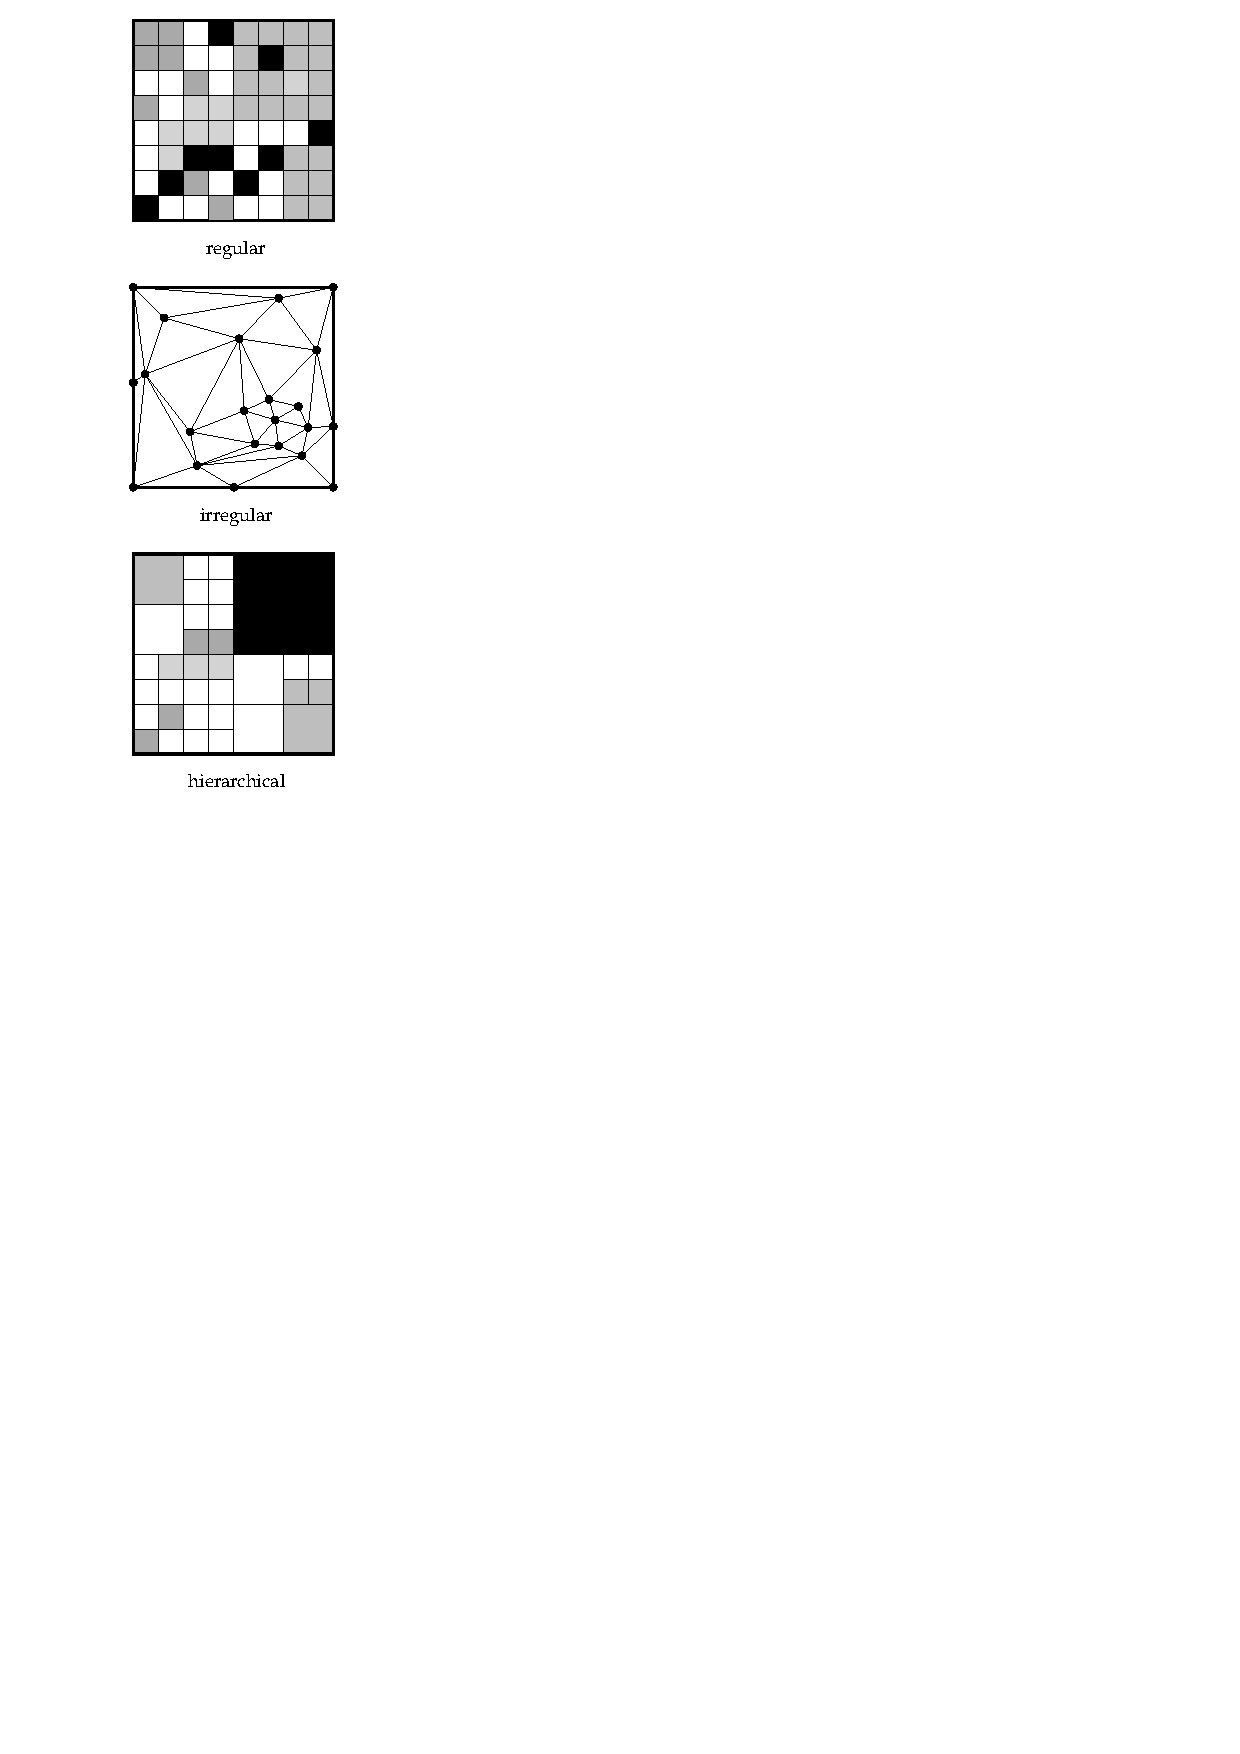
\includegraphics[width=0.7\textwidth]{figs/tesstype}
  \caption{Type of tessellations.}% 
\labfig{fig:tesstypes}
\end{marginfigure}

%

Piecewise models typically imply that a supporting data structure is constructed, and stored, to represent the tessellation.
% (it is however possible to construct on-the-fly some well-known structures only when they are needed since they have formal rules).
Some of these tessellations partition arbitrarily the space, while some are based on the spatial distribution of the sample points.


%%%
%
\section[Data models for terrains]{Data models for representing terrains in a computer}

\subsection{Spatial data models $\neq$ data structures}

In the GIS literature, there exists a confusion between the terms ``spatial model'' and ``data structure''. 
The confusion originates from the fact that object and field views of space are usually implemented in a GIS with respectively vector and raster models. 
However, this is not always the case as TINs can be used for fields for instance.
A ``spatial data model'' offers an \emph{abstract} view of a data structure, it is an abstraction of the reality.
A data structure is the specific implementation of a spatial data model, and deals with storage, which topological relationships are explicitly stored, performance, etc.
The same spatial data model can therefore be implemented with different data structures.



%%%
\subsection{Regular Tessellations} 

As shown in \reffig{fig:tesstypes}a, all the cells have the same shape and size.
The most common regular tessellation in GIS and in terrain modelling is by far the grid (or raster representation), in which the cells are squares in 2D (usually called \emph{pixels}, a portmanteau of `picture' and `element', as an analogy to digital images).
However, while they are not common in practice, other regular shapes are possible, such as hexagons or triangles.

%

Observe that a regular tessellation often arbitrarily tessellates the space covered by the field without taking into consideration the objects embedded in it (the samples). 
This is in contrast with irregular tessellations in which, most of the time, the shape of the cells constructed depends on the samples.

In practice this means that, if we have a terrain stored as a regular tessellation we can assume that it was constructed from a set of samples by using spatial interpolation.
Converting sample points to cells is not optimal because the original samples, which could be meaningful points such as the summits, valleys or ridges of a terrain, are not necessarily present in the resulting tessellation. 
There is a loss of information, since the exact location of the meaningful points are lost.
% Also, when a practitioner has access to a grid, she often does not know how it was constructed and what interpolation method was used, unless meta-data are available.

%

\paragraph{Concrete example: a 2D grid.}
A 2D grid, stored for instance with the GeoTIFF format, is thus a piecewise representation of a 2D field: a regular tessellation where each cell has a constant function.
The value assigned to each cell is an estimation previously obtained by spatial interpolation.
However, for a given grid, it is usually unclear if the value of a cell is for its centre, or for one of its vertices (and if it is the case, for which one?).
Different formats have different rules, and converting a field represented with one format to another one (while retaining the same cell resolution and spatial extent) can shift the value from the centre to the top-left corner for instance.

%

The wide popularity of regular tessellations in terrain modelling is probably due to simplicity and to the fact that they permit us to easily integrate 2D remote sensing images and terrains.
Indeed, a grid is naturally stored in a computer as an array (each cell is addressed by its position in the array, and only the value of the cell is stored), and thus the spatial relationships between cells are implicit. 
This is true for any dimensions, thus, contrary to other tessellations, grids are very easy to generalise to higher dimensions.
The algorithms to analyse and manipulate (Boolean operations such as intersection or union) are also straightforwardly implemented in a computer. 

On the other hand, grids also suffer problems.
First, the size of a grid can become massive for data at a fine resolution; this problem gets worse in higher dimensions.
Second, grids scale badly and are not rotationally invariant, \ie\ if the coordinate reference system used is changed, then the grid needs to be reconstructed to obtain regular cells whose boundaries are parallel to the axes of the reference system.
To assign a new value to the transformed cells, spatial interpolation is needed, which is often performed not by re-using the original samples, but by using the values of the neighbouring cells.
Unfortunately, each time a grid is transformed its information is degraded because not the original samples are used, but interpolated values.



%%%
\subsection{Irregular Tessellations} 

The cells of an irregular tessellation can be of any shape and size, and they usually `follow'---or are constrained by---the samples points that were collected, albeit this is not a requirement. 
Subdividing the space based on the samples has the main advantage of producing a tessellation that is \emph{adaptive} to the distribution of the samples. 
The subdivision is potentially better than that obtained with regular tessellations (which subdivide arbitrarily the space without any considerations for the samples).

%

The most known examples of the use of irregular tessellations in terrain modelling is the \emph{triangulated irregular network}, or TIN\@.%
\index{TIN}\marginnote{TIN: triangulated irregular network}

As shown in \reffig{fig:tin}, a TIN refers to an irregular tessellation of the $xy$-plane into non-overlapping triangles (whose vertices are formed by three sample points), and to the use of a linear interpolation function for each triangle. 
\begin{marginfigure}
  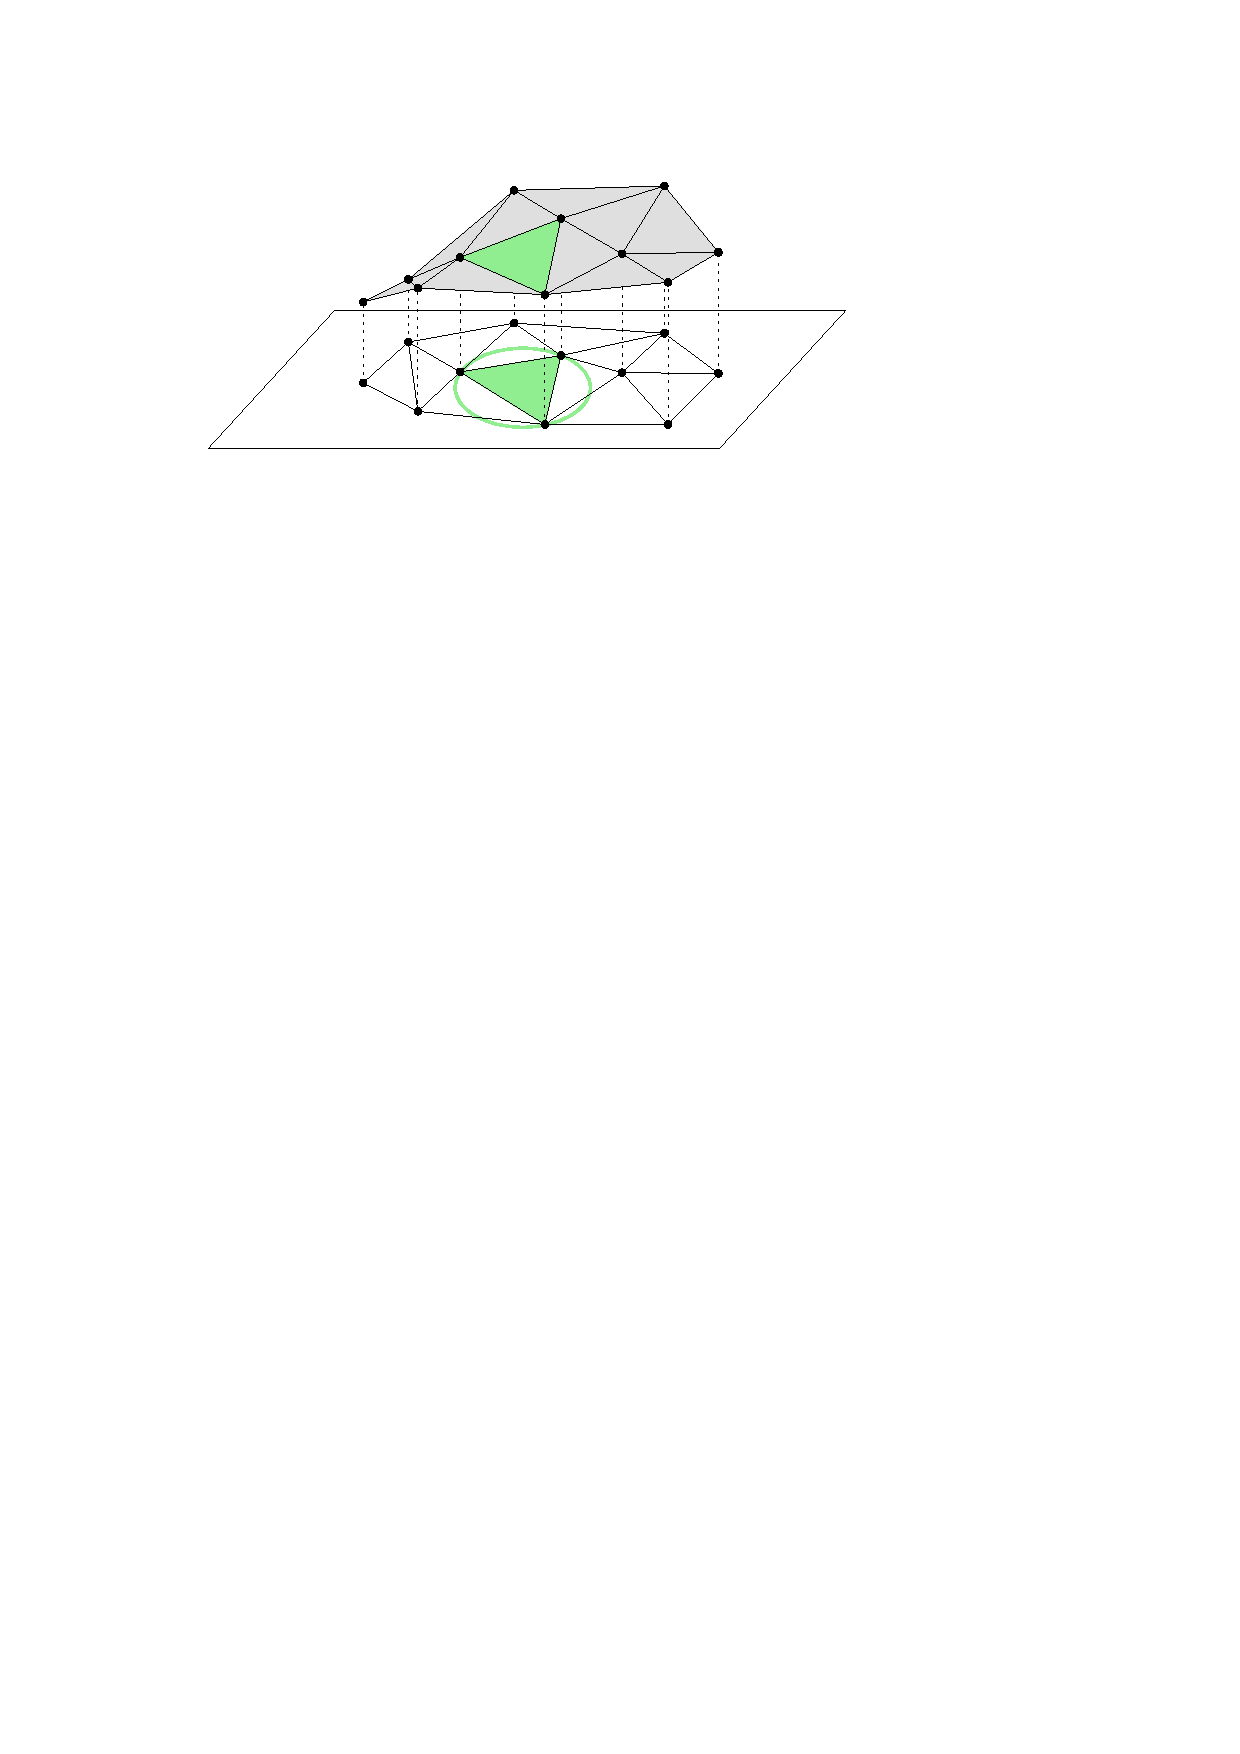
\includegraphics{figs/tin}
  \caption{A TIN is obtained by lifting the vertices to their elevation. All the triangles are usually Delaunay, \ie\ their circumcircle (green) is empty of any other points in the plane.}%
\labfig{fig:tin}
\end{marginfigure}
One way to explain the 2.5D properties of a TIN is as follows: if we project vertically to the $xy$-plane the triangles in 3D space forming the TIN, then no two triangles will intersect.

While not a requirement, the triangulation is usually a Delaunay triangulation (more about this in Chapter~\ref{chap:dtvd}).
The main reason is that Delaunay triangles are as ``fat'' as possible (long and skinny triangles are avoided), and thus they behave better for interpolation.
As can be seen in~\reffig{fig:whydt},
\begin{figure}
  \centering
  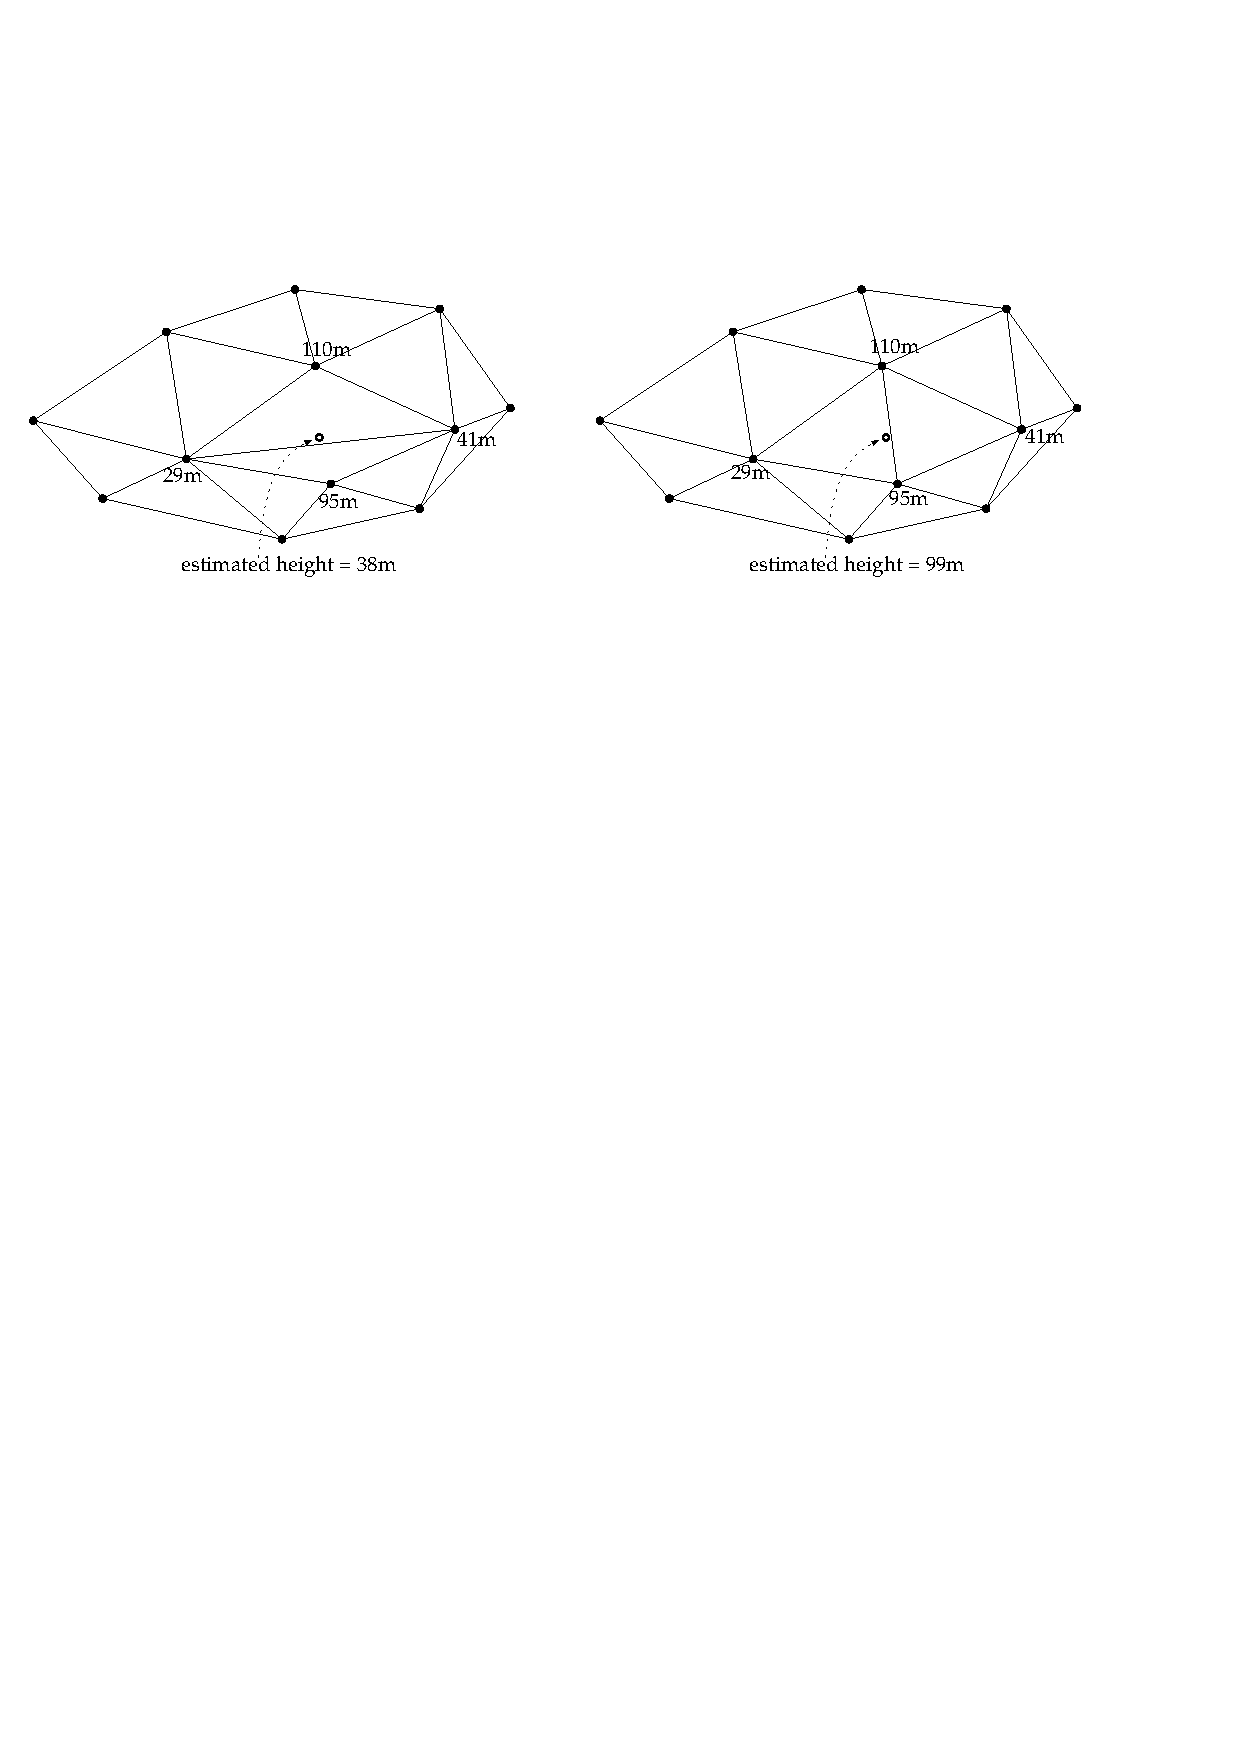
\includegraphics[width=\linewidth]{figs/whydt}
  \caption{Two TINs (left is a DT, right has one non-Delaunay edge) and the result of estimating with linear interpolation in the TIN\@.}%
\labfig{fig:whydt}
\end{figure}
the estimated value can be significantly different, and in this case the right one would make more sense since sample points that are closer to the interpolation location are used (in the TIN on the left, the value of 95m is not used).

%

Each of the points (which becomes vertices in the triangulation) are lifted to its elevation to create a surface, embedded in three dimensions, approximating the morphology of the terrain.
The value of elevation at an unsampled location $p$ is obtained by linearly interpolating on the plane passing through the three vertices of the triangle containing $p$. 
TINs are the most popular alternatives to 2D grids for modelling elevation; both representations have advantages and disadvantages.

%
 
A TIN in which a linear interpolation function is used yields a $C^0$ piecewise representation, \ie\ it is a continuous function but at the edges of the triangles the first derivative is not possible.
It is possible to use higher-order functions in each triangle of a TIN, to construct a $C^1$ or $C^2$ field, \ie\ where the first and second derivative of the surface can be obtained. 
Chapter~\ref{chap:interpol} gives more details.



%%%
\subsection{Hierarchical tessellations}

Hierarchical tessellations attempt to reduce the number of cells in a tessellation by merging the neighbouring cells having the same value (thus yielding cells of different sizes).
While both regular and irregular tessellations can be hierarchical, in the context of the representation of terrains, the former is more relevant and is sometimes used in practice.

% Irregular hierarchical tessellations, usually triangulations, are used for obtaining multi-resolution models, or act as a spatial index for efficiently accessing triangles.
% Their use as a support to construct a piecewise function is not necessary because irregular tessellations have cells of different sizes and shapes.
% Consequently, only hierarchical regular tessellations are discussed in the following.

%

A commonly used hierarchical structure in two dimensions is the \emph{quadtree}, which is a generic term for a family of tessellations that recursively subdivide the plane into four quadrants.%
\index{quadtree}\marginnote{quadtree}
As is the case for grids, quadtrees are relatively easily implemented in a computer because they are trees in which each node has exactly four children, if any.

%

The shortcomings of regular hierarchical tessellations are similar to those of regular tessellations: the rotation and scaling operations are difficult to handle.
The main advantage of using them---saving memory space---is present only when there is spatial coherence between cells having the same attribute value, \ie\ when they are clustered together.
Indeed, the size of a quadtree is not dependent on the number of cells, but on their distribution.
The quadtree of a 2D grid having no two adjacent cells with the same value (\eg\ a checkers board) contains the same number of cells as the grid, and its size would most likely be worse because of the overhead to manage the tree.
Another disadvantage is that the notion of neighbours, which is straightforward in regular tessellations, is less trivial.


%%%
\subsection{Other common terrain representations used in GIS}

\begin{marginfigure}
  \centering
  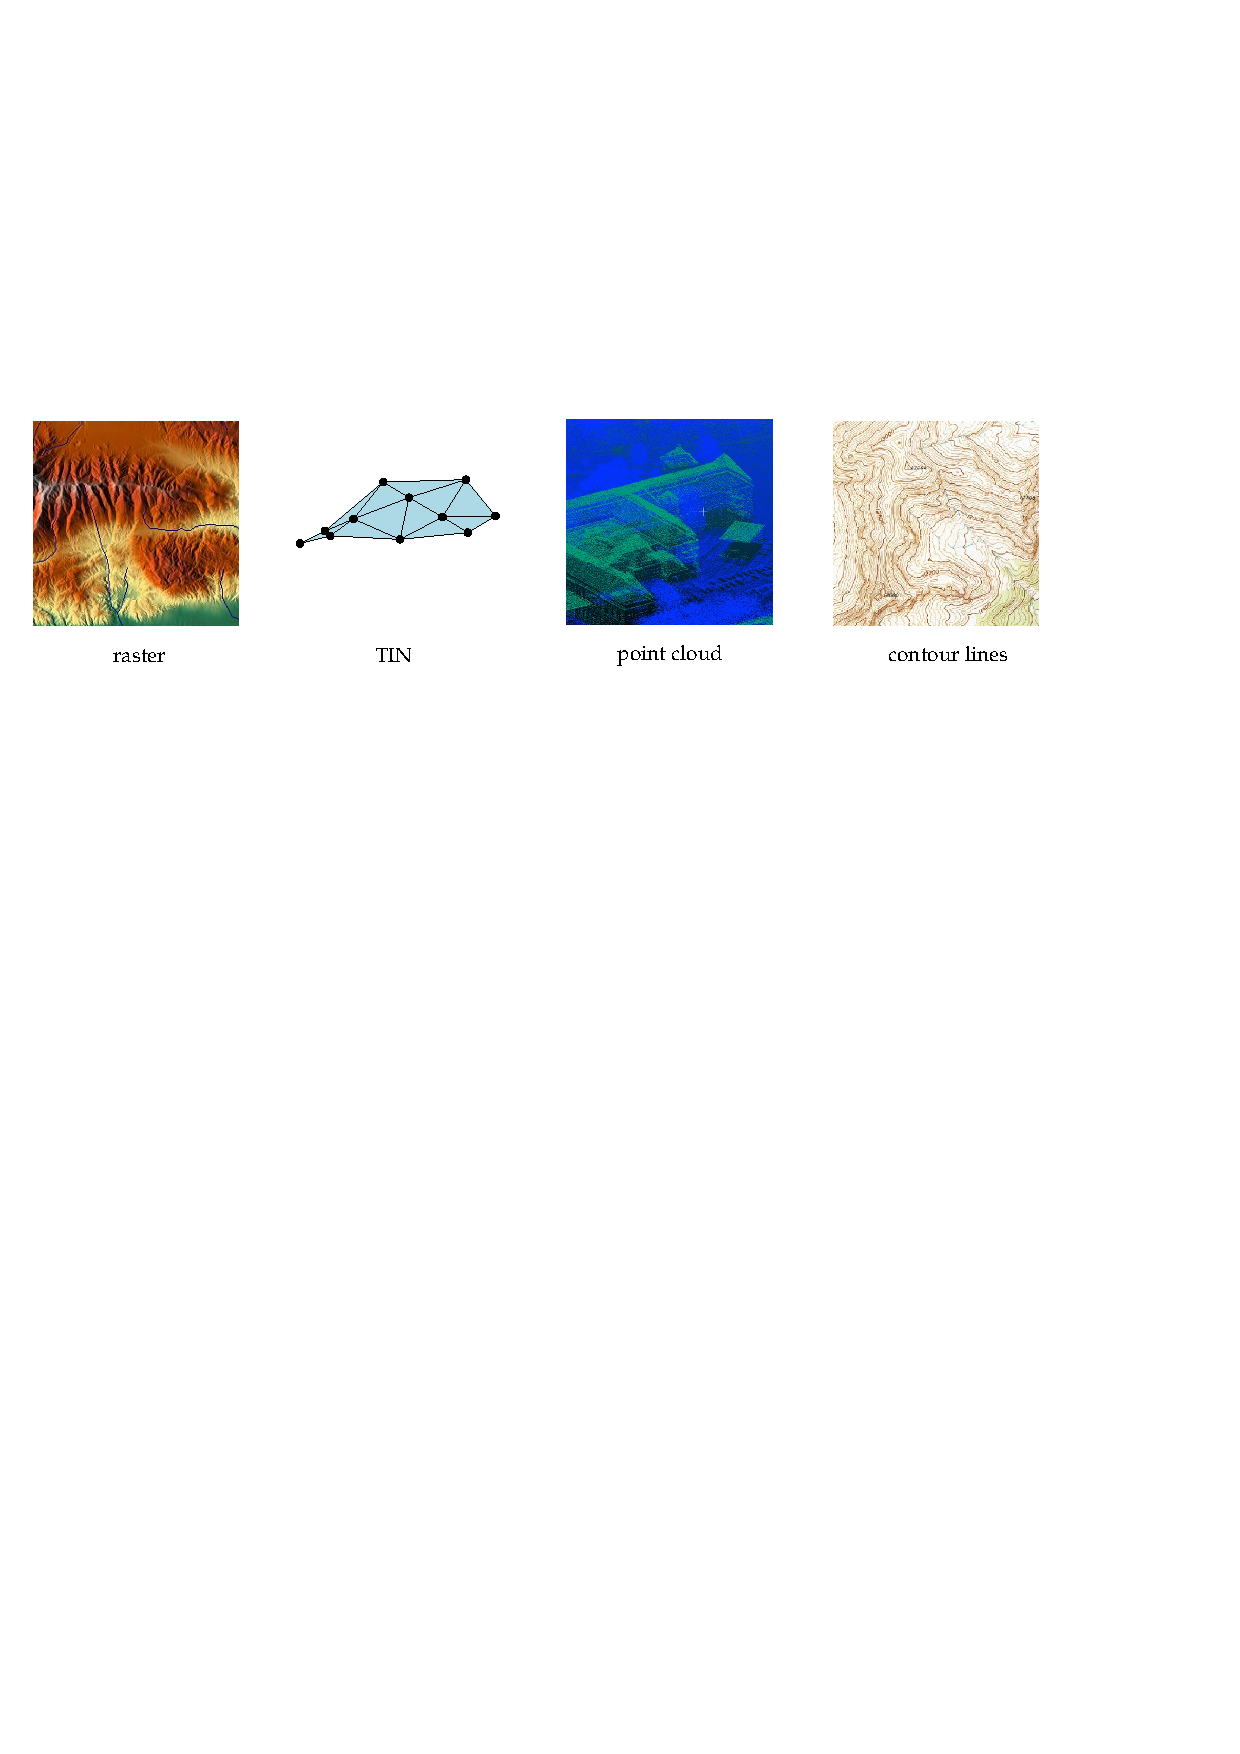
\includegraphics[width=0.75\linewidth]{figs/reps}
  \caption{Four most common data models for terrains.}%
\labfig{fig:reps}
\end{marginfigure}

In the GIS literature, besides the ones above, different representations for terrains are often listed, the two most relevant being:
\begin{enumerate}
  \item irregularly spaced sample points, such a point cloud; 
  \item contour lines.
\end{enumerate}
It should be noticed that these two are however \emph{incomplete}: the set of rules to reconstruct the surface at unsampled locations is not explicitly given, they are not continuous surfaces.
Conceptually speaking, these should therefore not be considered valid representations of a terrain.
While this might seems odd, this is in line with the consensus among practitioners today, where a point cloud or contour lines would typically be used as an input to a process to generate a terrain.

We will nevertheless consider these in the course; the four representations we will use are shown in \reffig{fig:reps}.

%

\paragraph{Contour lines.}%
\index{isolines}\index{contour lines}

Given a bivariate field $f(x,y) = z$, an \emph{isoline} (commonly named contour line) is the set of points in space where $f(x,y) = z_0$, where $z_0$ is a constant. 
Isolines have been traditionally used to represent the elevation in topographic maps and the depth in bathymetric maps for navigation at sea. 

%

% TODO : change the nicked contour example jpg? Remove it?
\begin{marginfigure}
  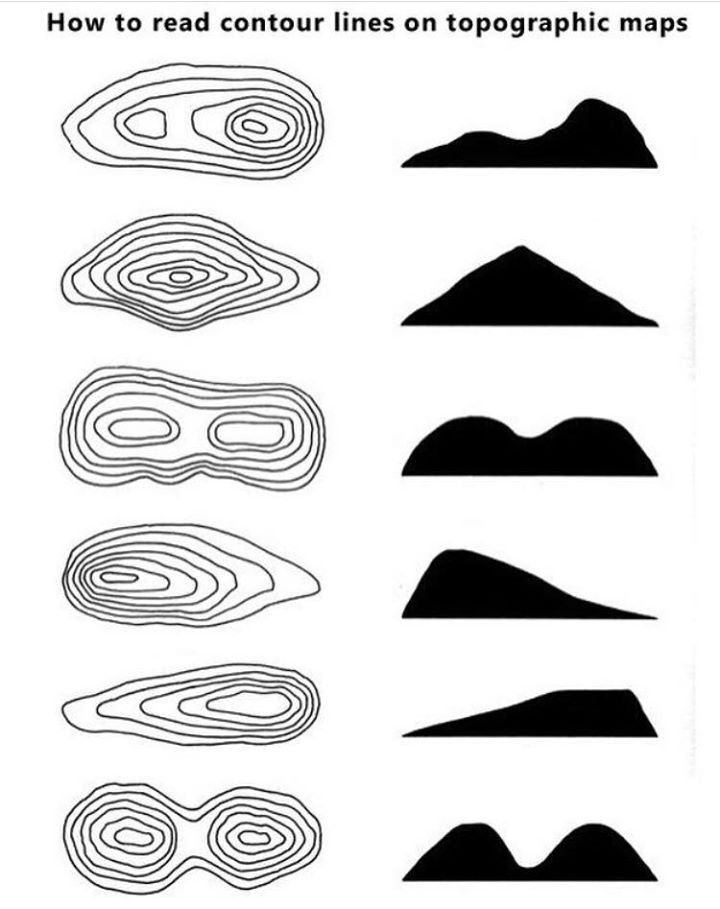
\includegraphics{figs/contours.jpg}
  \caption{A few examples of terrain features and their contour lines. (Figure from \citet{Kjellstrom99})}%
\labfig{fig:contours}
\end{marginfigure}

One particular property of an isoline is that its direction is always perpendicular to the direction of the steepest slope of the terrain. 
Another property that follows from the $2.5D$ property of the field is that contours neither intersect themselves nor each other.

%

The purpose of isolines on a map is to reveal the shape of the underlying terrain. 
By observing the shape and interrelation of neighbouring contours, the presence and significance of surface features becomes apparent; see~\reffig{fig:contours} for a few examples.
It should be noticed that data between contours is absent in the contour map. 
Yet, in case of good contours the reader will still be able to deduct the general morphology of the field. 
It is even so that the use of contours will speed up the map reading process, as it conveys just that relevant bit of data to the map reader rather than `flooding' the reader with information which essentially makes the user do his own cartographic selection. 
Contouring is a form of discretizing the field that makes it easier to use a map. 
Naturally, this comes at a price. 
The level of approximation of the field can (dramatically) differ between contours, the biggest error would be midway in between contour lines. 
But, depending on the relation between the spacing between contours (the \emph{contour interval}) and the map scale, which in turn is dependent on the map application, this effect may be neglected.


%

In practice, isolines are only approximated from the computer representation of a field.
They are usually extracted directly from a TIN or a regular grid. 
As shown in~\reffig{fig:isoline},
\begin{figure}
  \centering
  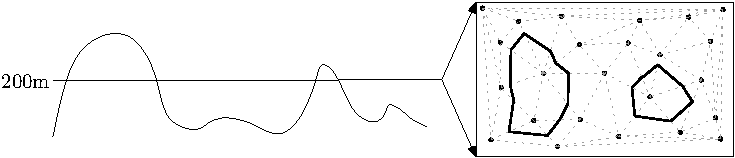
\includegraphics[width=0.95\textwidth]{figs/isoline}
  \caption{Cross-section of a terrain (left), and the 200m isoline extracted from a TIN (right).} 
\labfig{fig:isoline}
\end{figure}
the idea is to compute the intersection between the level value (\eg\ 200m) and the terrain, represented for instance with a TIN\@. 
Each triangle is scanned and segment lines are extracted to form an approximation of an isoline.
Chapter~\ref{chap:conversion} gives more details.

%%%
%
\section[TIN versus raster]{TIN versus raster for modelling terrains}

There is an ongoing debate about whether TINs or rasters are the better data model to model terrains.
Practitioners and scientists are probably split 50/50 on the issue.

A data model will be judged more \emph{efficient} than another if it represents a surface more accurately within the same amount of storage space, measured in bytes.
This of course depends on the data structure used to store that data model.

It should be said that both TIN and raster have advantages and disadvantages (as we will see during this course), and in practice one should choose the most appropriate model for the task at hand.
This means converting between the two data models when it is necessary (topic of \refchap{chap:conversion}).


%%%
%
\section{Notes and comments}

\citet{Kumler94} carried out a 4-year comparison between TINs and rasters.
He states that the common belief that a TIN is more space-efficient than raster is handicapped by the fact that a TIN must have \emph{at least} 3 times less points to be of equal space.
His conclusions are also that rasters can estimate elevation more accurately than comparably-sized TINs.
However, he still finishes with by stating: ``Yeah, well\ldots\ TINs still \emph{look} better.'' 

\citet{Fisher97} discusses the disadvantages of rasters, in a GIS and remote sensing context.

\citet{Frank92,Goodchild92a} discuss at lenght the issue of data model, data structure and representation of reality. 

\citet{Tse04} coined the term `2.75D GIS' and show an example of a where a triangulation is used to represent the surface of the Earth, with holes (for tunnels), cliffs and caves. 
The same idea is also referred to as a `2.8D GIS' by \citet{Groger05}.

While more an academic exercise then something used in practice, multi-resolution triangulation have been described and used for some application by \citet{DeFloriani02}.

\citet{Akima78} shows the advantages of using higher-order functions in each region of a TIN, to construct a $C^1$ or $C^2$ field. 

\citet{Dakowicz03} demonstrate that using simple rules (nearest-neighbour for instance) yields fields that are not realistic and have bad slope, which is in practice problematic for several applications.
Obtaining good slope from contour lines is possible, but is in practice a complex process.
% In other words, if elevation is the attribute modelled, the slope of the terrain will be `good', which is important for several applications, for example flood modelling.


%%%
%
\section{Exercises}

\begin{enumerate}
  \item Explain in our own words why a point cloud (\eg\ collected with airborne lidar) is not considered a complete representation of a terrain.
  \item What is a bivariate function? 
  \item Assume you have 2.75D terrain of an area. Is it possible to extract the isolines from it? What properties will these have? Will they intersect?
\end{enumerate}
